\documentclass[11pt]{article}
\usepackage{graphicx}
\usepackage{timeline}
\usepackage{cite}
\usepackage[hang,small,bf]{caption}
\usepackage{booktabs}
\usepackage{chngpage}
\usepackage[toc,page]{appendix}
\renewcommand{\thefootnote}{\fnsymbol{footnote}}
\newcommand{\ra}[1]{\renewcommand{\arraystretch}{#1}}

\usepackage{textcomp}
\bibliographystyle{unsrt}

\begin{document}

\title{Master's thesis proposal [rev\_4]}
\author{\normalsize Richard Oldham, DDS \vspace{7pt} \\ 
		\small University of Pittsburgh \vspace{-2pt} \\
		\small Department of Biomedical Informatics}
\maketitle


\begin{abstract}
The benefits of Computerized Patient Records (CPRs) are well documented. Yet current dental CPRs inadequately support chairside use. If dental professionals have any hope of realizing the advantages of CPR use, information systems must adapt to their workflow and not \textit{vice versa}. To that end, research suggests tablet devices hold promise as an alternative to traditional desktop PCs' ergonomic shortcomings in the clinical environment. Designing a tablet-based treatment planning application for the clinician may help bridge the adoption gap between office and chairside computer use in dentistry. Evaluation can determine if users are faster, more successful, or more subjectively satisfied with the tablet application over traditional CPRs.
\end{abstract}

\section{Background}
First, I summarize applicable findings from informatics research on CPRs. Next, I discuss a user model for treatment planning in dentistry. Lastly, I discuss conclusions and potential solutions.

\subsection{Adoption and Usability}

The adoption of Computerized Patient Records (CPRs) by healthcare professionals has long been recognized as a key step in improving patient care\cite{Chasteen1992A-computer-data,Eisne1993The-computer-ba,Thompson2004The-Decade-of-H,Spicer2008Bytes-and-bites,Schleyer2011Advancing-oral}. Dentists recognized the power of computers assisting with practice administration --- such as scheduling and billing --- becoming early adopters of computers in-office (Figure 1).
\label{fig:1}
\begin{figure}[!h]
\begin{center}
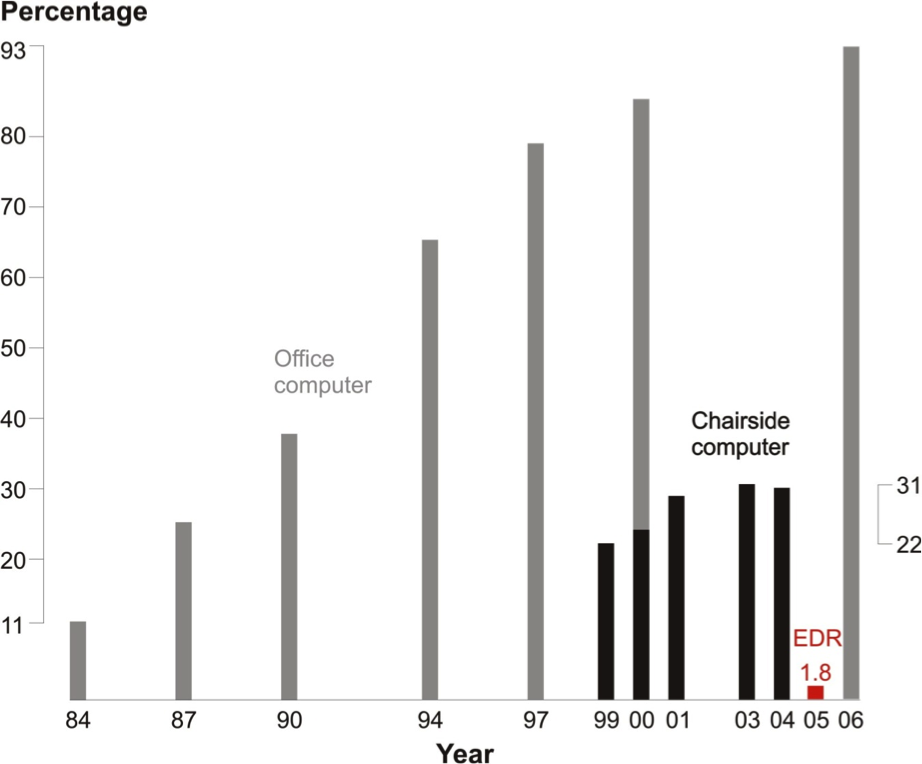
\includegraphics[width=\textwidth]{comp.png}
\end{center}
\caption{Year of first computer installation for office and chairside use by US dentists\cite{Schleyer2006Clinical-Comput}. The red bar represents completely paperless practices.}
\end{figure}
\newpage

\noindent Survey data from 2010, the most recent available, reported 92\% of respondents using Practice Management Software (PMS)\cite{Levine2010}.\footnote[2]{Here I use PMS to refer to software that handles office administration whereas a CPR handles patients' clinical data. Most CPR software is also PMS but not the other way around.} However, the conclusions of two usability studies on four dental CPRs, which together comprise more than a 70\% market share for such systems, suggest poor usability is a barrier to dental CPR adoption for chairside use\cite{Thyvalikakath2007Heuristic-evalu,Thyvalikakath2008A-usability-eva}. The gap between office adoption of computers and the adoption of computers for chairside use is evident in Figure 1.

The first of the two cited usability studies employed heuristic evaluation methods\cite{Nielsen1994Usability-Inspe}. Three expert reviewers examined each of the four CPRs and tabulated violations of Nielsen's heuristics \cite{Thyvalikakath:2009fk}. Evaluators found 229 heuristic violations in total across EagleSoft, Dentrix, PracticeWorks, and SoftDent suggesting the software dentists were using at the time had significant room for usability improvement. The second usability study compared\cite{Nielsen1994Enhancing-the-e} these same market-leading CPRs by assigning common tasks to novice users and measuring task completion. On average, users were able to correctly complete 43\% of the assigned tasks leading to a similar conclusion: the most commonly used dental CPRs suffered from a steep learning curve and unintuitive interface design.

The results of these two studies point to inadequate support for chairside use. All four systems included in these studies began life as PMS with clinical functions added later. Nested menus and tree selections for clinical items alongside similarly organized non-clinical functions are evidence of this. Such input selection is far from efficient in an environment that requires efficiency. All four systems evaluated by Thyvalikakath et al. employ screen designs that include nearly all input options at once rather than the options needed for the specific task or goal (Figure 2). Interfaces with many options make finding the function of interest more difficult, increase cognitive load, and slow the user\cite{Qian2011Towards-develop}. Dentrix and Eaglesoft screen design, for example, confused novice users with intermixed controls for entering existing conditions and planned procedures on the same palette.
\label{fig:2}
\begin{figure}[h!tb]
\begin{center}
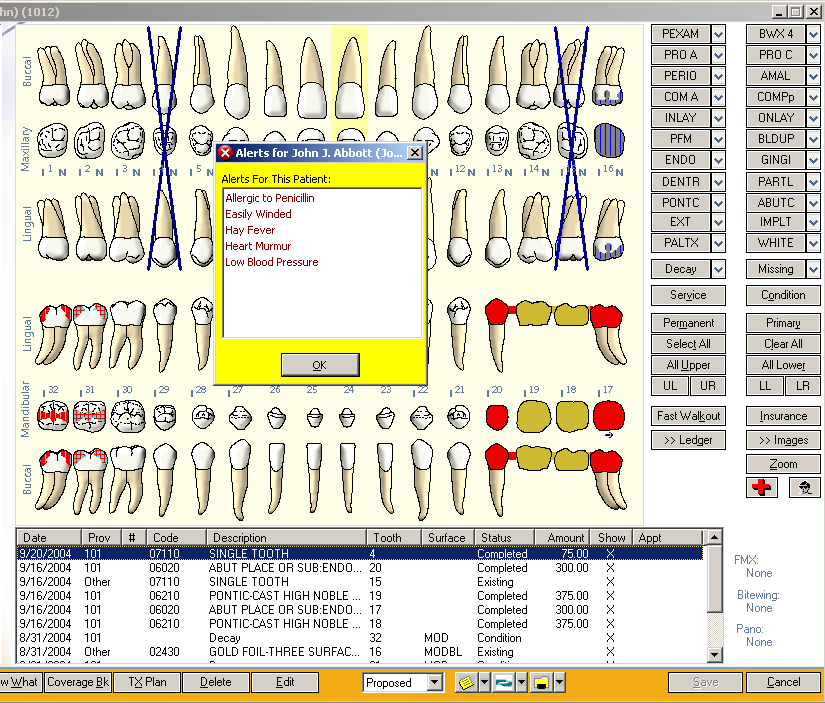
\includegraphics[width=\textwidth]{ss1es.png}
\end{center}
\caption{Screenshot of EagleSoft's user interface.}
\end{figure}Since the information input and retrieval processes are not integrated into the concepts of tasks and workflow, users must divide their attention between navigation and task completion. In both usability studies, the authors noted information that would typically appear on a single paper form was spread out over two or more screens in the CPR. The comparative evaluation study cited difficulty with tasks that required screen switching as a principle source of user frustration. Evidence suggests these problems are not unique to dental health information technology (HIT) applications\cite{Ash2004Some-unintended,Rose2005Using-qualitati}.

\subsection{Attitudes and Use}
In a telephone survey of 102 general dentists in the United States, researchers discovered two main sources of user frustration in using dental CPRs: steep learning curves and difficulty entering clinical data\cite{Schleyer2006Clinical-Comput}. Respondents considered `better input methods,' `smaller computers,' and `better user interface design' as principal areas for improvement. Another important concern included lack of infection control inherent with traditional keyboard and mouse input. These responses track closely with those elicited from British users through a similar survey\cite{John2003Questionnaire-s}.

%The Dental Information Model (DIM), a blueprint for the content and structure of patient records in general dentistry, is maturing through research collaboration between the Center for Dental Informatics and Marshfield Clinic Biomedical Informatics Research Center\cite{Acharya2009Electronic-dent}. The DIM offers guidance for database design in helping ensure the software system has adequate expressive power\cite{Schleyer2007A-Qualitative-I} in making real world data elements to data fields in the system. Doing so could address the disconnect between the real world and system noted in usability testing and survey data on what types of data are stored on paper and the computer. Further, data interchange is made easier in using a standard DIM. To the extent the interface design must dovetail with the underlying data layer, the DIM is helpful in designing the interface as well.

Dental practices use their computers primarily for scheduling patients and tracking completed procedures (Figure 3).\label{fig:3}
\begin{figure}[!t]
\begin{center}
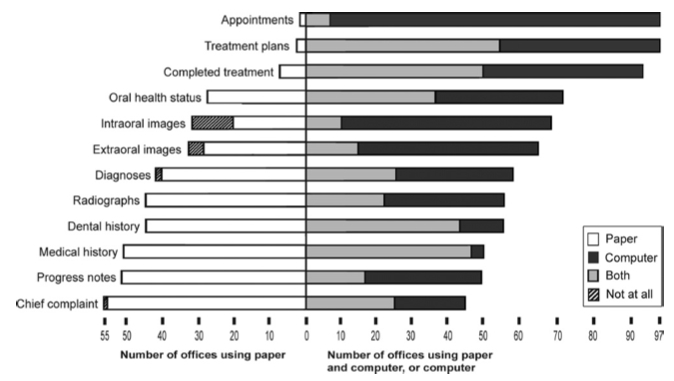
\includegraphics[width=\textwidth]{papervscomp.jpg}
\end{center}
\caption{Storage of major clinical information categories on paper/computer, sorted by utilization of computer-based storage in descending order\cite{Schleyer2007A-Qualitative-I}.}
\end{figure}
Because dental CPRs are poorly designed for chairside use, some users accommodate by working around the CPR. Some practices record temporary notes on a patient napkin or tray cover and commit these notes to the electronic record later while others record histories on paper and treatments on the computer. While transcribing notes from paper to the computer is not an inherent problem, such a practice has the potential for error. Storing some information in paper format and some in electronic format (Figure 3), similarly, is not \emph{prima facie} poor practice but requires the consumer of the information to switch between the paper-based and computer-based records. Fragmentation of data into multiple locations has one inevitable drawback: switching requires the user to remember which piece of information is needed and where this information is located. This cognitive burden can slow the consumption of information by the clinician or produce transcription errors\cite{Salvucci2009Toward-a-unifie}. The need to work around the CPR is due, in some part, to the difficulty of integrating the necessary hardware into an already cramped dental operatory\cite{Schleyer2004Why-integration,Unthank2004Designing-your-} and, in some part, to the time-prohibitive cost of entering data into a poorly designed system. The ergonomics of one dentist, one assistant, and one patient gathering, entering, retrieving, and presenting information are complex. The suggested areas of improvement noted in the Schleyer, et al. (2006) survey highlight the frustration of using software designed without these ergonomics in mind. The task of finding the required information inside the patient record is often criticized as time-intensive and distracting\cite{Nygren1998Helping-clinici}. This is especially concerning given the increased complexity of care provided in an increasingly time-pressured environment. If we accept the premise that HIT can improve patient care, and there exists a large adoption gap, the necessity of generating and understanding a user model becomes apparent.

\subsection{User Model}
Recognizing this adoption gap, researchers set out to model the workflow of an initial examination and treatment planning appointment through contextual inquiry\cite{Irwin2009A-preliminary-m}. During this appointment the dentist documents the patients current condition, the patient-specific goal for oral health, and generates a sequenced plan to proceed from present state to the goal state. This process, with its findings and resulting plan, must then be discussed with the patient. Depending on the complexity of diagnoses, multiple treatment plans may be required. Of any appointment, this one generates the most clinical artifacts such as radiographs, hard and soft tissue diagnostic charting,  and study models. Following the initial visit and generation of a treatment plan, each subsequent visit requires comparatively little interaction with the CPR. The dentist may check the medical history or reference the planned procedures, for example. Thus the initial appointment requires the most interaction with the CPR for data entry and retrieval, making it an ideal candidate for study.

A thorough initial exam and treatment planning appointment is vital for not only diagnosing every present condition but communicating the condition, its consequences, and treatment options as well. Generating a treatment plan is analogous to peeling an onion: the dentist starts with the most obvious signs and symptoms and continues examination, testing, and imaging until all signs and symptoms have been mapped to a problem list. The dentist may ascribe diagnoses to items on the problem list and then generate a treatment to address each item. This process is non-deterministic, across patients and dentists, and time-intensive, often requiring two people. Typically one operator will diagnose and call out findings while an auxiliary transcribes the findings into the computerized record. While this task may be handled differently in sequence from one dentist or patient to another, the steps are the same and mappable to common set of terms and abstractions. 

Irwin, et al. (2009) observed an auxiliary may not always be available and dental team members used a variety of workarounds in such a situation. For example, hygienists often perform recare examinations without an assistant, noting their preliminary findings on a piece of paper prior to discussion with the dentist. Some clinicians postpone any data entry tasks to a time after the patient has been dismissed. This presents the problem of having to remember what was done and why. Even under ideal circumstances, that is, when an assistant was present, over 60\% of the Irwin's observed breakdowns were due to technology. One implicit conclusion from the Irwin model was dentists spend little time entering data with the majority of CPR interaction handled by hygienists and assistants. Schleyer, et al. (2006) reported dentists participating in only 23\% of data entry tasks, chief among them being progress note entry. Hygienists and assistants handled most other data entry tasks such as diagnoses, oral health status, and histories. Whether dentists would employ more clinical functions in their CPR given improved interfaces, as Irwin, et al (2009) described, ``with the flexibility in sequencing, granularity and comprehensiveness'' for data entry remains to be seen. But Irwin conclusions mirror the conclusions from the Schleyer et al. 2006 survey: CPR design must accommodate to the demands of dental workflow.

Schleyer et al. (2006, 2007) and Irwin et al. (2009) report the common practice of using multiple or duplicate data entry. A user may write something on paper, such as routing slips or preliminary findings, later transcribing this information into the electronic record. Alternatively, a practice may record the medical history on paper and use the CPR to record planned and completed treatments. This is due, in part, to the fact that dental CPRs lack some date elements and the flexibility present in paper forms\cite{Schleyer2007A-Qualitative-I}. And, in part, to the non-linear and variable process by which patients are escorted through this initial visit. Therefore, an alternative system needs to allow the user a temporary and mutable data store to enter information before committing the entry to the record. And the clinical vocabulary of the information system must be at least as large as that of the clinician. While one can never hope to \emph{a priori} enumerate this vocabulary, allowing the user to customize the type and sequence of information capture may suffice. 

\subsection{Conclusions and Solutions}
Several important conclusions can be gleaned from the cited literature. First, dental operatories are small and require careful planning to integrate the CPR's supporting hardware. The suggestion of using smaller computers from the Schleyer, et al. (2006) survey reveals user frustration with this integration burden. Next, the current paradigm in dental CPR design and ergonomics requires an auxiliary for efficient data entry. Most dentists are consumers of patient information while hygienists and assistants perform most data entry. Following the generation of a treatment plan, subsequent appointments require comparatively little data entry or retrieval. Given the results of the user model study, the highest value targets for CPR improvement are the functions used during the initial visit: namely, diagnoses and treatment planning. Lastly, CPRs are poorly adapted to dental workflow and most dental teams accommodate by using multiple or duplicate data entry. For over a decade, dental clinicians have recognized the potential for hand-held computing devices to address the limitations of traditional PCs\cite{Taylor2002Handheld-comput,Jablow2003Your-practice-i}. Given the findings from survey data, usability studies, and contextual inquiry, a paradigm shift is necessary.


\section{Tablets and Usability}
Tablets offer several advantages over traditional desktop PCs in clinical use. Because CPR access is not universally available in medical exam rooms, tablets' smaller size and portability were central to their adoption by physicians. Tablets' allow the clinician to enter orders, notes, and review information while remaining mobile. Likewise, tablets' smaller footprint and portability could address the ergonomic challenges in dental practice. A tablet is ideal for consuming information, which is the principle concern of the clinician. Tablets can at least match the traditional desktop PC in data entry speed and accuracy with use\cite{Kirby1996The-PEN--PAD-da,Mackenzi2002Text-entry-for-}. They can be easily shared between the provider and patient and easily disinfected\cite{Mayrhofer2007Pen-based-Elect}. Properly designed touch-screen mobile interfaces have demonstrated promise in a variety of medical settings\cite{Haller2009Handheld-vs.-la,Mulligen1998Clinical-data-e,Baumgart2005Personal-digita,Lu2005A-review-and-a-,Seneviratne2010Improving-stylu}. Finally, if users are as capable on a mobile device as a traditional PC, the ergonomic and portability advantages can increase user subjective satisfaction with a mobile system over a conventional desktop\cite{Cole2006A-comparative-s}.

Some remain skeptical of the virtues of tablet computers in clinical use\cite{Kaneshige2011iPad-in-Healthc,Mashman:2011uq} and, compared to the medical literature, few investigators have studied tablet use by the dental team\cite{Frank2010IPad--tool-or-t}. Applying the insights from medical informatics research to dental problems presumes exchangeability of the domains. This may not be the case. Physician and dentist workflows have differences (Table 1). \begin{table}[h!t]
	\caption{Summary comparison of differences across medicinal and dental domains}
	\begin{adjustwidth}{-.5in}{-.5in}
	\begin{center}
	\ra{1.3}
\begin{tabular}{l  l  l}
\toprule
\makebox[0.32\textwidth][r]{\textbf{Feature of practice}} & \makebox[0.3\textwidth][r]{\textbf{Domain}}	\\	
\cmidrule{2-3}	& \textit{Dentistry} 	& 	\textit{Medicine} \\ 
\midrule
Patient status				&  Usually not sick	&  Usually sick      \\
Life and death encounters	&  Seldom			&  More often        \\
No. of encounters per day	&  Few				&  Many              \\
No. of diagnoses			&  Few				&  Many              \\
No. of therapies per diagnoses	&	Many 		&  Few               \\
No. of initial visit artifacts	&	Many 		&  Few               \\
Average visit length			&	Long 		&  Short             \\
\bottomrule
\end{tabular} \end{center} \end{adjustwidth} \end{table}
A key difference to note is the small number of diagnoses in dentistry compared to medicine; dentists cover a smaller portion of the body compared to physicians. Conversely, for each diagnoses, there are a larger number of choices for treatment in dentistry compared to medicine. One might explain this difference by pointing to the larger role patient preferences play in dental treatment planning\cite{Kay1992Restorative-tre} or the smaller role of evidence-based practice in dentistry compared to medicine\cite{Tellez-2011-Sealants}. Another key difference is ergonomic: physicians stand or sit bedside while the dental ergonomic is unique. However, given the success enjoyed by tablets in complex medical settings, I remain optimistic about tablet performance in the dental operatory. Creating a usable and useful interface for the tablet is a separate consideration.

Regarding screen design, Thyvalikakath, et al. (2008) recognized the disconnect between task flow and screen design in dental CPRs ahead of a formal modeling study. Several topical conclusions the 2008 comparative usability study include: \begin{itemize}
\item Users should be able to identify their treatment preferences and software should support that approach.
\item Data entry and retrieval controls available on screen should correspond with the tasks to be completed. Unrelated or extraneous controls should not be shown. Information that belongs to a specific task context should be shown together or be easily accessible. For instance, hard-tissue and periodontal findings often must be reviewed together to make a clinical decision and should not be separated unnecessarily.
\item Data entry and functional controls should be organized and labeled clearly according to input class (findings, planned/completed procedures, notes, pictures, annotations, etc.).
\end{itemize}

Lastly, the User-Centered Design (UCD) approach to software engineering has demonstrated promise in general\cite{Bannon1986Issues-in-desig,Wixon1997The-usability-e,Gould1997How-to-design-u,Abras2004Encycolopeida-o} and HIT specifically\cite{Johnson2005A-user-centered}. UCD is a broad term to describe design processes in which end-users influence the software design. Linking the iterative design process to feedback from users has a proven track record of producing highly usable software. I elaborate on the proposed incorporation of the UCD approach in section 3.2.

\section{Proposed Research}
Based on research evidence, tablet devices make a logical hardware choice. However, hypotheses about tablet use in dentistry remain untested. The extent to which tablet devices and touch interfaces can improve data entry and user satisfaction is a question left to evaluation. But first an interactive tablet-based treatment planning prototype is needed.

Research is currently underway to qualify and quantify the data private practice dentists capture in their CPRs. Given the time constraints of clinical practice and poor usability demonstrated by market-leading CPRs, we hypothesize dentists predominantly document completed procedures and few diagnostic findings (Figure 3). This is accepted practice by third-party payers, in contrast to medicine. Given the lack of open-domain knowledge of type and quantity of data users store, design choices must rely on literature and best practices. But once completed, the data from this study can help inform system design --- ranked list UI elements, for example.

I propose testing two hypotheses: (1) tablet computers, using platform-native UIs, can at least match conventional desktop computers in data entry speed and task completion; (2) users will prefer using a mobile touch screen device over the conventional desktop PC.

\subsection{Treatment Planning Prototype}

To effectively evaluate the comparative usability of tablets and desktop PCs a measure of functional equivalence across the two systems is required. That is to say the tablet prototype requires the ability to input and retrieve the same clinical artifacts necessary for treatment planning as a mature software system like Dentrix of EagleSoft. Such artifacts include:
\begin{itemize}
\item Patient histories: both medical and dental histories are critical to patient safety and disease management
\item Hard tissue: both existing work and conditions that would indicate treatment
\item Soft tissue: periodontal measures such as clinical attachment level, soft tissue margins, and common periodontal findings
\item Picture Archival and Communication System: radiographs as well as intraoral and extraoral photographs play an increasingly important role in dental practice. Such artifacts provide not only valuable information to the clinician for decision-making but also aid in communicating the same information in a patient-friendly manner.
\end{itemize}
These are the same class of items required to work through case examples in the seminal textbook on dental treatment planning by Sefanic and Nesbit\cite{Stefanac2006Treatment-Plann}. Further these artifacts are the same ones used by non-digital dentists and correspond with the task and user models generated by Irwin \textit{et al.}, thus offering a consensus for high value targets for data input and retrieval. Assuming the four mentioned artifacts are necessary and sufficient to complete a dental treatment plan, and given that such functionality is already present in current CPR vendor offerings, what is the value proposition?

From survey data we know that dental practices value data entry related to financial reimbursement. Poor usability demonstrated in evaluation offers a plausible explanation for this. Why would a clinician bother with the many clicks and screen shuffling required to document all of their findings in the record if they are paid only for the completed treatments? If a system were designed with goals and tasks in mind, however, it is feasible that a small number of rules could unambiguously and programatically render diagnoses from problems---generating knowledge from data. By providing an incentive to enter data more complete patient data we can both improve data quality and save the user time.

During my training it was often repeated that my job was not to fill teeth but to diagnose disease. From contextual inquiry it is evident that many dentists become overwhelmed by the workday and adopt a treatment minded mental heuristic. Instead of asking ``why is there pathology present'' many dentists skip to ``what treatment should address the problem?'' A new paradigm in software would accompany the clinician through the exam offering the appropriate prompts to drill down to diagnoses from problems.

%Many options are available for mobile development. The two dominant operating systems for tablet devices are Android and iOS. To develop a platform-native application, Android requires application coding in Java and iOS requires coding in Objective-C. Alternatively, a web-native application can be ``wrapped'' for use on any platform using responsive web design (a small JavaScript instruction set to resize content based on browser resolution). While each platform has advantages and disadvantages, no design decision has yet been made.

In order for the prototype to be interactive, The functional specification includes:

\begin{itemize}
\item The ability to document the most common diagnostic findings in a clinically linear fashion (find all sites affected with diagnostic condition, move on to the next condition)
\item The ability to automatically generate diagnoses from the documented findings
\item The ability to automatically map a list of treatments, based on provider preferences, from the list of problems and diagnoses
\item The ability to bin and sequence the list of treatments to form one or several treatment plans
\end{itemize}

Following the generation of a treatment plan (or plans), the provider next discusses the findings with the patient. The ability to summarize findings for the providers use in treatment planning is as important as communicating these findings to the patient. Using the treatment plan ``patient view'' to facilitate this discussion could help drive treatment plan acceptance. This feature would undoubtedly be beneficial but may fall outside the scope of this project. The ``patient view'' function is but one example of the many functions available to users once patient data is present in the CPR. However, addressing the problem of cumbersome data entry is a necessary prerequisite to reaping the benefits of computerized records.

\subsection{Evaluation}

Evaluation of the tablet application requires comparing it to an alternative. Two logical points of comparison are the most popular CPRs in private practice: Dentrix and EagleSoft. Access to these CPRs has been granted to the CDI and using them for the purposes of evaluation should present no challenges.

Similar to Thyvalikakath, et al. (2008), summative measures like task completion provides a valuable evaluation metric. Task completion time and subjective user satisfaction are also useful\cite{Chin1998Development-of-}. Task completion time can be simply measured with a stop watch by an observer. Subjective user satisfaction could be measured through a survey administered after each user completes the task set on each system. By using within-subjects comparison the effect of user familiarity with tablet devices and the traditional CPR can be minimized. A pre-observation survey of user comfort and familiarity with the two systems may help explain differences across users. 

One important tradeoff to consider is fidelity to real-world use versus ease of evaluation. Setting up a mock clinic with myself (or someone else) acting as a patient would provide a more realistic environment but may bias the evaluation if the primary investigator serves also as the mock patient. Alternatively, several na\"{i}ve users could complete a common task set using the tablet application and an alternative.

As previously described, the UCD approach to development is ideally suited to the proposed research. The University of Pittsburgh's Center for Dental Infromatics and School of Dental Medicine can provide ready access to potential participants for design feedback ahead of the formal evaluation. The purpose of this feedback is to confirm the design specification and to maximize application usability. Depending on the results of this feedback, one or more rounds of iteration may be necessary.  

\section{Proposed Timeline}



\begin{timeline}{4.2in}(5,265)
\optrule
  \item[10]{April}{Initial proposal}
  \item[14]{April}{Begin thesis}
  \item[18]{May}{Begin development}
  \item[52]{June}{Begin contextual inquiry}
  \item[92]{August}{Complete contextual inquiry}
  \item[102]{August}{Model building}
  \item[102]{August}{Begin sketches and paper prototypes}
  \item[112]{September}{Screen design and wireframe revision}
  \item[112]{September}{Preliminary expert review}
  \item[132]{September}{Complete preliminary expert review}
  \item[160]{September}{Complete proposal}
  \item[163]{September}{Complete functional specification}
  \item[170]{October}{Begin principal development}
  \item[195]{October}{Second round of expert review}
  \item[202]{November}{Begin design iteration}
  \item[226]{December}{Third round of expert review}
  \item[230]{December}{Design polish}
  \item[250]{January}{Complete interactive prototype}
  \item[257]{January}{Begin evaluation}
\end{timeline}%% Needed comment
\newpage

\footnotesize{
\bibliography{Master}}
\newpage

\appendix
\renewcommand\thesection{Appendix \Alph{section}}

\section{Physical Models}
\subsection{Rear-delivery}

\begin{figure}[h!t]
\begin{center}
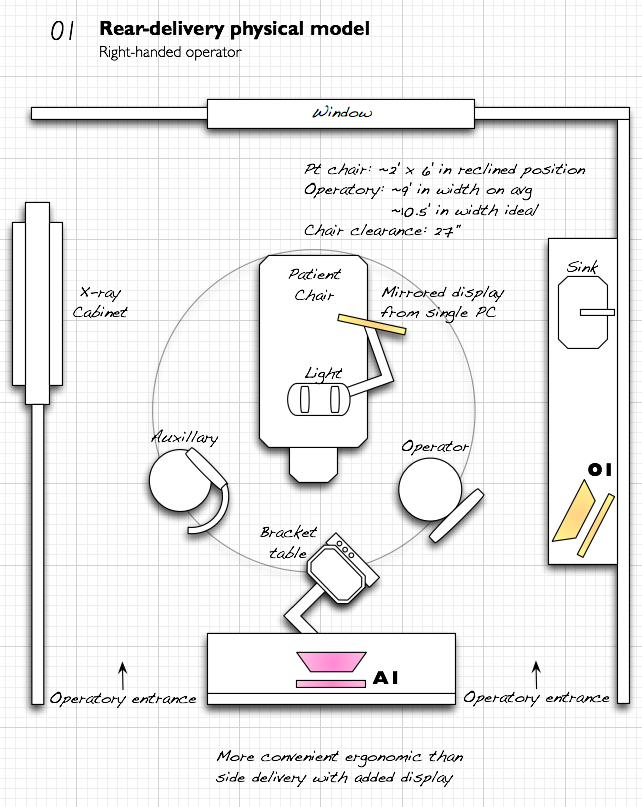
\includegraphics[width=\textwidth]{phymodel1.png}
\end{center}
\caption{Rear-delivery physical model for a right-handed operator.}
\end{figure}

\subsection{Side-delivery}
\begin{figure}[h!]
\begin{center}
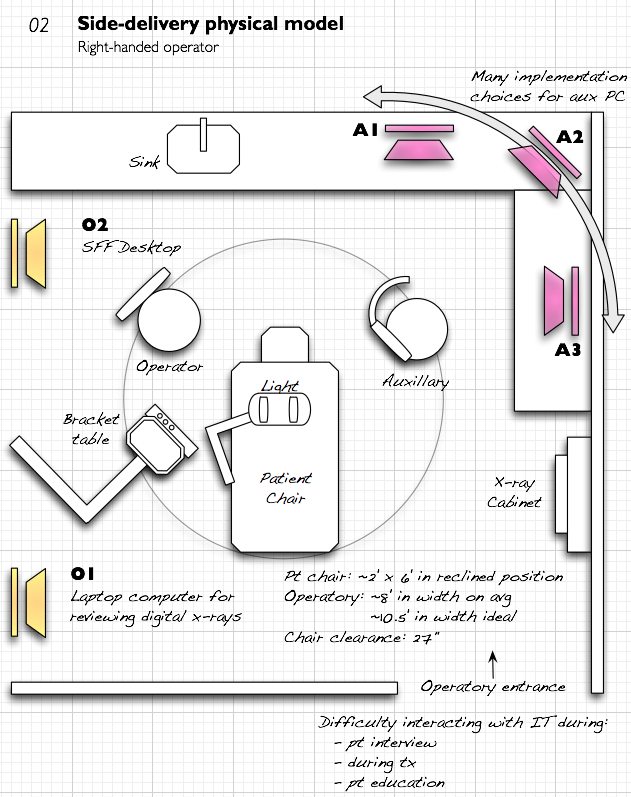
\includegraphics[width=\textwidth]{phymodel2.png}
\end{center}
\caption{Side-delivery physical model for a right-handed operator.}
\end{figure}

\newpage


\section{Artifact Model}
\begin{figure}[h!b]
\begin{center}
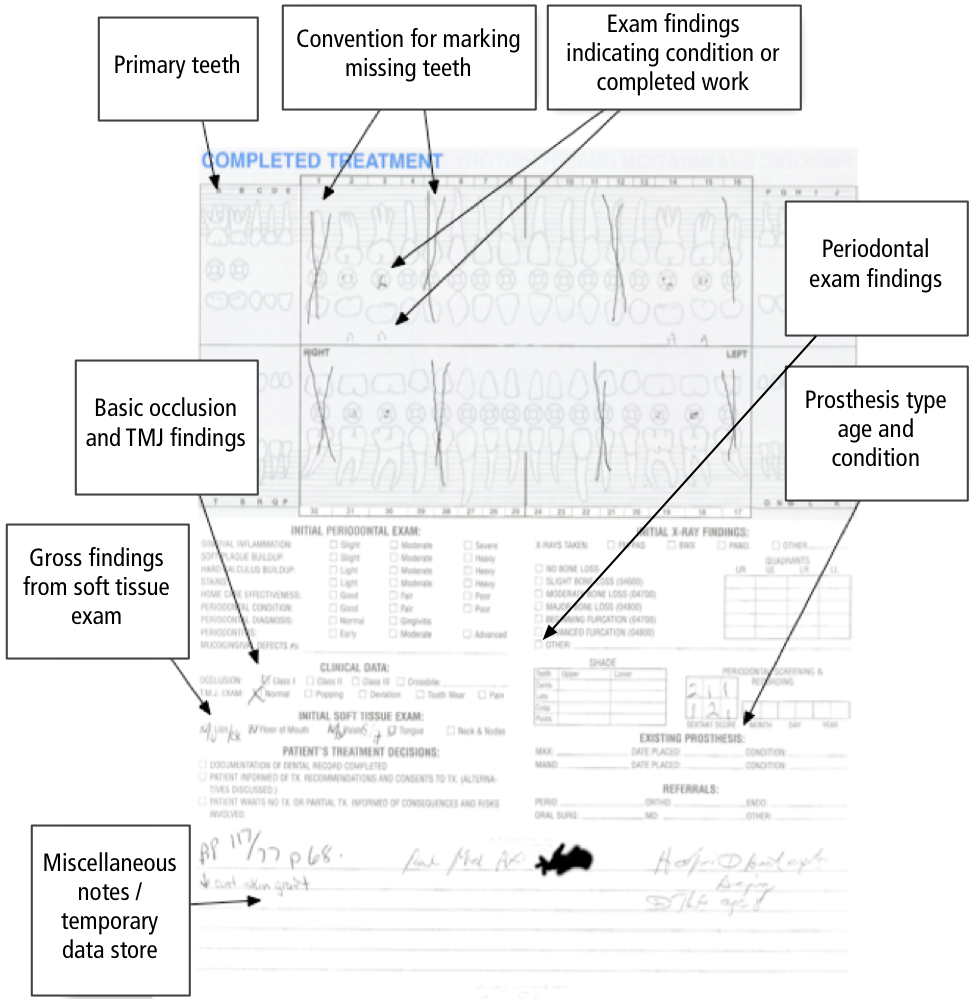
\includegraphics[width=\textwidth]{artifactmodel.png}
\end{center}
\caption{Artifact model generated from common paper-based treatment planning forms}
\end{figure}


\end{document}	